\documentclass{article}
% PACKAGES
\usepackage[english]{babel}
\usepackage{graphicx} % Required for inserting images
\usepackage[most]{tcolorbox}
\usepackage{lmodern}
\usepackage{titlepic}
\usepackage{pdfpages}
\usepackage{tcolorbox}
\usepackage{amsmath}
\usepackage{pgfplots}
\usepackage{xcolor}
\usepackage{tikz}
\usepackage{color,soul}
\usepackage{enumerate}
\usepackage{enumitem}
\usepackage{cancel}
\usepackage{hyperref} 
\usepackage{tikzsymbols}
\usepackage{fontawesome5}
\usepackage[export]{adjustbox}
\usepackage{amssymb}
\usepackage{tikz,lipsum,lmodern}


% COLOURS
\definecolor{Orchid}{RGB}{218, 112, 214}
\definecolor{snow}{rgb}{1.0, 0.98, 0.98}
\definecolor{mordantred19}{rgb}{0.68, 0.05, 0.0}
\definecolor{mistyrose}{rgb}{1.0, 0.89, 0.88}
\definecolor{nadeshikopink}{rgb}{0.96, 0.68, 0.78}
\definecolor{cadmiumgreen}{rgb}{0.0, 0.42, 0.24}
\definecolor{OliveGreen}{RGB}{85, 107, 47}
\definecolor{RoyalPurple}{RGB}{120, 81, 169}
\definecolor{NavyBlue}{RGB}{0, 0, 128}
\definecolor{CornflowerBlue}{RGB}{100, 149, 237}
\definecolor{Cerulean}{RGB}{0, 123, 167}
\definecolor{DarkOrchid}{RGB}{153, 50, 204}

\title{MCV4U - Calculus}
\author{Kensukeken}
\date{9 February 2024}

\begin{document}
\maketitle

\tableofcontents
\newpage
\section{Unit 2}
\subsection{Instantaneous Rate of Change, aka Tangent Lines, Slope at a Point, Derivatives}
\underline{Tangent Lines:} A tangent line to a curve is the straight line that most resembles the graph near that point.  By finding the slope of a tangent line, we can find the slope of the curve at the given point. \\ \\ 
Here are some examples of tangent lines:

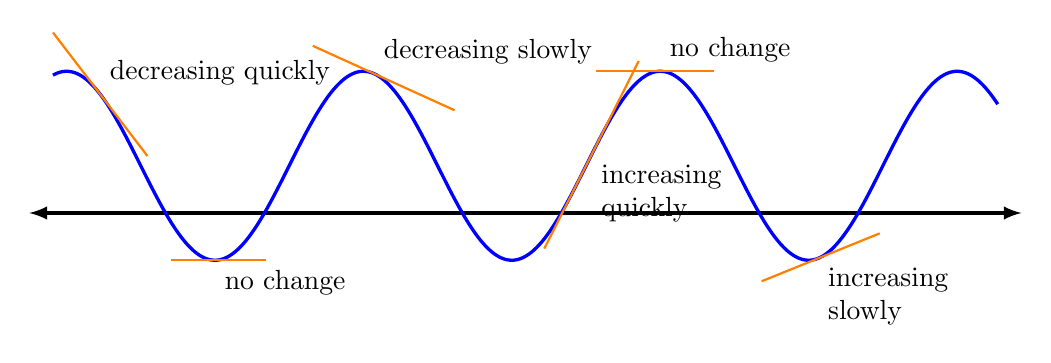
\begin{tikzpicture}[scale=0.6]
  \draw[latex-latex, very thick] (-5.5,0)--(15.5,0);

  \draw[domain=-5:15,samples=200,smooth,variable=\x, blue, very thick] plot ({\x},{1+2*sin(\x r)});
 
  \draw[domain=-5:-3,smooth,variable=\x, orange, thick] plot ({\x},{2*\x*cos(4 r) + 1 - 2*sin(4 r) + 8*cos(4 r)});
  \node[above right] at (-4,{1+2*sin(-4 r)}) {decreasing quickly};
 
  \draw[domain=-2.5:-.5,smooth,variable=\x, orange, thick] plot ({\x},{1+2*sin(-1.57 r)});
  \node[below right] at (-1.57,{1+2*sin(-1.57 r)}) {no change};
 
  \draw[domain=0.5:3.5,smooth,variable=\x, orange, thick] plot ({\x},{3.76562-0.4544*\x});
  \node[above right] at (1.8,{1+2*sin(1.8 r)}) {decreasing slowly};
 
  \draw[domain=5.4:7.4,smooth,variable=\x, orange, thick] plot ({\x},{1.98637*\x - 11.4797});
  \node[below right,text width=2cm] at (6.4,{1+2*sin(6.4 r)}) {increasing quickly};
 
  \draw[domain=6.5:9,smooth,variable=\x, orange, thick] plot ({\x},{1+2*sin(7.85 r)});
  \node[above right] at (7.85,{1+2*sin(7.85 r)}) {no change};
 
  \draw[domain=10:12.5,smooth,variable=\x, orange, thick] plot ({\x},{0.40601*\x - 5.50566});
  \node[below right,text width=2cm] at (11.2,{1+2*sin(11.2 r)}) {increasing slowly};
\end{tikzpicture}
Up until now, we have talked about needing two points to determine the slope of a line. However, as we begin talking about derivatives, we need to talk about the slope of a curve at a certain point. \\
Suppose that we wish to determine the slope of the curve $y=f(x)$ at the point where $x=a$. This is the same as finding the slope of the line tangent to the curve $y=f(x)$ at $x=a$.\\
When $x=a$, $y=f(x)$.  Therefore, we will be trying to determine the slope of the curve $y=f(x)$ at the point $(a, f(a))$.
    \begin{figure}[ht]
    \centering
    \includegraphics[width=0.6\textwidth]{imgs/slopoftangent.png}
    \end{figure}
\begin{tcolorbox}[colback=Orchid!5!white,colframe=Orchid!75!white,coltitle=white,title=Slope of Tangent ]
The derivative of the function $y=f(x)$ is given formula
  \[
  f'(x)=\lim_{h \to 0} \frac{f(x+h)-f(x)}{h},
  \]
 Other symbols for the derivative include $y'$ and $\frac{\delta y}{\delta x}$
\end{tcolorbox}
The derivative of a function allows you to determine the slope of the line tangent to a curve at a given point. In other words, you can find the slope of the line when you only know one point on the line. The value of the derivative is often called the instantaneous rate of change.
\subsubsection*{Example:}
Determine the derivative of the function $y=x^2$ and evaluate the derivative at the point where $x=3$.\\ \\ 
\textbf{Solution:}
\begin{align*}
    y' &= \lim_{x \to 0} \frac{f(x+h)-f(x)}{h}\\
    &= \lim_{h \to 0} \frac{(x+h)^2-x^2}{h}\\
    &= \lim_{h \to 0} \frac{x^2+2xh+h^2)-x^2}{h}\\
    &= \lim_{h \to 0} \frac{2xh+h^2}{h}\\
    &= \lim_{h \to 0} (2x+h)\\
    &= 2x + 0\\
    &= 2x.\\
    & \therefore y'=2x, \text{ at } x=3. \\
    y' &=2(3)=6 
\end{align*}
By evaluating the limit as the change in \( x \) approaches zero, we find the derivative \( y' = 2x \). Therefore, at \( x = 3 \), the derivative equals 6.
\newpage
\subsubsection*{Example:}
Determine the equation of the tangent line to the curve $y=x^2$ at the point where $x=3$. \\ \\ 
\textbf{Solution:}
\begin{align*}
    y &= mx + b, \quad \text{we know } m = 6 \\
    y &= 6x + b \\
    & \text{Substitute }(3, 9): \\
    9 &= 6(3) + b \\
    -9 &= b \\
\end{align*}
Therefore, the equation of the tangent at \(x = 3\) is \(y = 6x - 9\).
\subsubsection*{Example:}
Give that $y=3x^2-7x+6$, determine the value of $\frac{\delta y}{\delta x}$ at $x=5$. \\ \\ 
\textbf{Solution:}
\begin{align*}
    f'(x)&=\lim_{h to 0} \frac{f(x+h)-f(x)}{h}\\
    &=\lim_{h to 0} \frac{3(x+h)^2-7(x+h)+6-(3x^2-7x+6)}{h}\\
    &=\lim_{h to 0} \frac{3(x^2+2xh+h^2)-7x+7h+6-3x^2+7x-6}{h}\\
    &=\lim_{h to 0} \frac{\cancel{3x^2}+6xh+3h^2\cancel{-7x}+7h\cancel{+6}\cancel{-3x^2}\cancel{+7x}\cancel{-6}}{h}\\
    &= \lim_{h to 0} \frac{6hx+3h^2-7h}{h}\\
    &= \lim_{h to 0} \frac{\cancel{h}(6x+3h-7)}{\cancel{h}}\\
    &=6x+3(0)-7\\
    &= 6x-7
\end{align*}
At $x=5$ 
\begin{align*}
    &\frac{\delta y}{\delta x}=6(5)-7\\
    &=23
\end{align*}
\newpage
\subsubsection*{Example:}
Determine the equation of the tangent line of the curve $f(x)= \frac{1}{x}$ at the point where $x=2$.\\ \\ 
\textbf{Solution:}
\begin{align*}
    f'(x) &=\lim_{h \to 0}\frac{f(x+h)-f(x)}{h}\\
    &=\lim_{h \to 0}\frac{\frac{1}{x+h}-\frac{1}{x}}{h}\\
    &=\lim_{h \to 0} \frac{\frac{x}{x(x+h)} -\frac{(x+h)}{x(x+h)}}{h}\\
    &=\lim_{h \to 0} \frac{x-(x+h)}{xh(x+h)}\\
    &=\lim_{h \to 0} \frac{x-x-h}{xh(x+h)}\\
    &=\lim_{h \to 0} \frac{\cancel{h}}{x\cancel{h}(x+h)}\\
    &=\frac{-1}{x(x+0)}\\
    &=\frac{-1}{x^2}
\end{align*}
At $x=3$, $y=\frac{1}{2}$. Therefore, the point is $\left(2,\frac{1}{2}\right)$.\\
The derivative is $\frac{-1}{x^2}$. Therefore, the slope at $x=2$ is $\frac{-1}{2^2}=\frac{-1}{4}$
\begin{align*}
    &= y=mx+b\\
    &= y=\frac{-1}{4}x+b\\
    & \text{Sub in} \left(2,\frac{1}{2}\right)\\
    \frac{1}{2} &= \frac{-1}{4}(2)+b\\
    1 &=b
\end{align*}
The equation of the tangent line is $y=-\frac{1}{4}x+1$
\newpage 
\subsubsection*{Example:}
Determine an equation of the line that is perpendicular to the tangent to the graph of $f(x)=\frac{1}{x}$ at the point where $x=2$ and that intersects it at the point of tangency.(this is called the normal) \\  \\ 
\textbf{Solution:}

Our point is still $\left(2,\frac{1}{2}\right)$, our perpendicular slope is the negative reciprocal of the $-1\frac{1}{4}$, which is 4.
\begin{align*}
    &\therefore y=4x+b\\
    &\text{sub in} \left(2,\frac{1}{2}\right)\\
    \frac{1}{2}&=4(2)+b\\
    \frac{-15}{2}&=b\\
\end{align*}
The equation of the normal is $y=4x-\frac{15}{2}$
\subsection*{The Existence of Derivatives:}
A function $f$ is said to be differentiable at $x=a$ if $f'(a)$ exists. At points where $f$ is not differentiable, we say that the derivative does not exist. Common ways for a derivative to not exist are shown.

\begin{figure}[h]
\centering
\begin{minipage}[b]{0.5\textwidth}
\centering
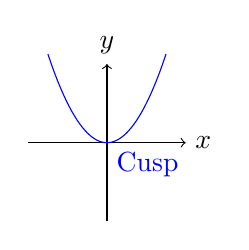
\begin{tikzpicture}[scale=0.5]
  % Cusp
  \draw[->] (-2,0) -- (2,0) node[right] {$x$};
  \draw[->] (0,-2) -- (0,2) node[above] {$y$};
  \draw[domain=-1.5:1.5, smooth, variable=\x, blue] plot ({\x}, {\x*\x});
  \node[below right, blue] at (0,0) {Cusp};
\end{tikzpicture}
\end{minipage}%
\begin{minipage}[b]{0.5\textwidth}
\centering
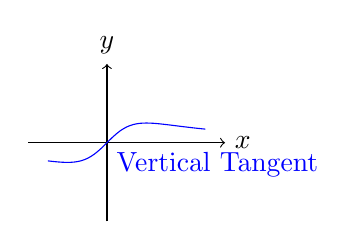
\begin{tikzpicture}[scale=0.5]
  % Vertical tangent
  \draw[->] (-2,0) -- (3,0) node[right] {$x$};
  \draw[->] (0,-2) -- (0,2) node[above] {$y$};
  \draw[domain=-1.5:2.5, smooth, variable=\x, blue] plot ({\x}, {\x/(1+\x*\x)});
  \node[below right, blue] at (0,0) {Vertical Tangent};
\end{tikzpicture}
\end{minipage}\\[20pt]
\begin{minipage}[b]{0.5\textwidth}
\centering
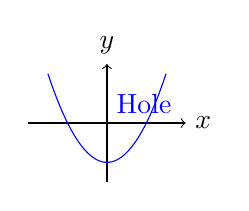
\begin{tikzpicture}[scale=0.5]
  % Hole
  \draw[->] (-2,0) -- (2,0) node[right] {$x$};
  \draw[->] (0,-1.5) -- (0,1.5) node[above] {$y$};
  \draw[domain=-1.5:1.5, smooth, variable=\x, blue] plot ({\x}, {(\x-1)*(\x+1)});
  \node[above right, blue] at (0,0) {Hole};
\end{tikzpicture}
\end{minipage}%
\begin{minipage}[b]{0.5\textwidth}
\centering
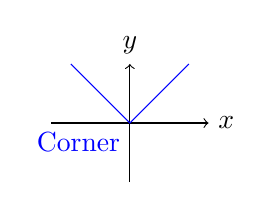
\begin{tikzpicture}[scale=0.5]
  % Corner
  \draw[->] (-2,0) -- (2,0) node[right] {$x$};
  \draw[->] (0,-1.5) -- (0,1.5) node[above] {$y$};
  \draw[domain=-1.5:1.5, variable=\x, blue] plot ({\x}, {abs(\x)});
  \node[below left, blue] at (0,0) {Corner};
\end{tikzpicture}
\end{minipage} 
\caption{Different Types of Discontinuities}
\label{fig:discontinuities}
\end{figure}

\section*{No Derivative}
\begin{minipage}[h]{0.7\textwidth}
  \centering
  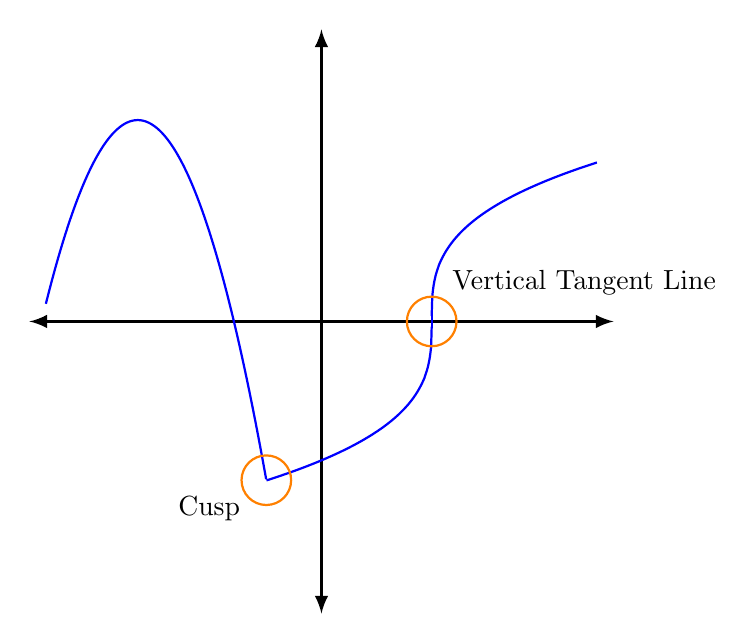
\begin{tikzpicture}[scale=0.7]
    \draw[latex-latex, very thick] (-5.3,0)--(5.3,0);
    \draw[latex-latex, very thick] (0,-5.3)--(0,5.3);
  
    \draw[domain=2.0001:5,samples=300,smooth,variable=\x, blue,  thick] plot ({\x},{2*exp(ln(\x-2)/3)});
    \draw[domain=2.0001:5,samples=300,smooth,variable=\x, blue,  thick,rotate around={180:(2,0)}] plot ({\x},{2*exp(ln(\x-2)/3)});
    \draw[blue,thick] (2,-0.1)--(2,0.1);
    \draw[domain=-5:-1,samples=300,smooth,variable=\x, blue,  thick] plot ({\x},-1.2*\x*\x-8*\x-9.68);
    \draw[orange,thick](-1,-2.88) circle (0.45);
    \draw[orange,thick](2,0) circle (0.45);
    \node[left] at (-1.3,-3.4) {Cusp};
    \node[above right] at (2.2,0.3) {Vertical Tangent Line};
  \end{tikzpicture}
\end{minipage}%
\begin{minipage}[t]{0.5\textwidth}
This graph represents a function that is not differentiable at certain points. The presence of a cusp and vertical tangent lines indicates that the function lacks a derivative at those points.
\end{minipage}

\section*{Inverse Derivative}
\begin{minipage}[h]{0.7\textwidth}
  \centering
  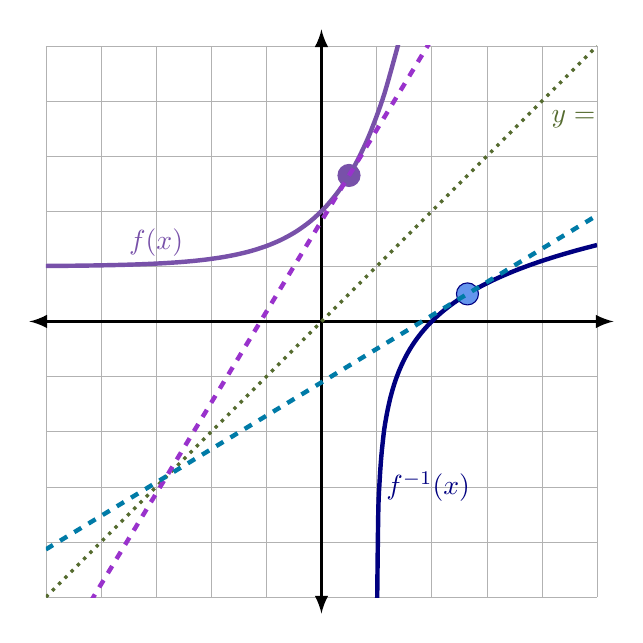
\begin{tikzpicture}[scale=0.7]
    \draw[black!30!white, very thin] (-5,-5) grid (5,5);
    \draw[latex-latex, very thick] (-5.3,0)--(5.3,0);
    \draw[latex-latex, very thick] (0,-5.3)--(0,5.3);
    
    \begin{scope}
        \clip (-5,-5) rectangle (5,5);
        \draw[very thick, OliveGreen,dotted](-5,-5)--(5,5);
        \node[OliveGreen,below right] at (4,4) {$y=x$};
        
        \draw[domain=-5:1.4,smooth,variable=\x, RoyalPurple, ultra thick] plot ({\x},{exp(\x)+1});
        \node[RoyalPurple,above] at (-3,1) {$f(x)$};
        \draw[RoyalPurple,fill=RoyalPurple] (0.5,2.649) circle [radius=0.2];
        \draw[domain=-4.5:2,smooth,variable=\x, DarkOrchid, ultra thick,dashed] plot ({\x},{1.649*\x+1.824});
        
        \draw[domain=1.003:5,smooth,variable=\x, NavyBlue, ultra thick, samples=150] plot ({\x},{ln(\x-1)});
        \node[NavyBlue,right] at (1,-3) {$f^{-1}(x)$};
        \draw[NavyBlue,fill=CornflowerBlue] (2.649,0.5) circle [radius=0.2];
        \draw[domain=-5:5,smooth,variable=\x, Cerulean, ultra thick,dashed] plot ({\x},{0.606*\x-1.105});
    \end{scope}
  \end{tikzpicture}
\end{minipage}%
  \vspace{2em}
\begin{minipage}[h]{0.5\textwidth}
This graph represents the inverse function of a function that has a derivative. The presence of a straight line indicates that the inverse function is linear. Additionally, the graph illustrates that the inverse function reverses the behavior of the original function with respect to the line $y=x$.
\end{minipage}



\subsection{Power Rule}
\begin{tcolorbox}[sharp corners=uphill,
    colback=purple!50!white,colframe=blue!25!black,coltext=yellow,
    fontupper=\Large\bfseries,arc=6mm,boxrule=2mm,boxsep=5mm]
  if $f(x)=x^{n}$, then $f'(x)=nx^{n-1}$
\end{tcolorbox}
  \textit{Proof}\\
  \begin{align*}
    f'(x)&=\lim_{h \to 0}\frac{f(x+h)-f(x)}{h}\\
    & \text{if } f(x)=x^n\\
    & \text{Then, } f(x+h)= (x+h)^n 
  \end{align*}
\subsubsection*{Example:}
if $f(x)= 4x^5$, then determine $f'(x)$. \\ \\ 
\textbf{Solution:}
\begin{align*}
    &= 4x^5\\
    &= (5)(4)x^{5-1}\\
    &=20x^4
\end{align*}
\subsubsection*{Example:}
if $f(x)= 11x^{\frac{5}{2}}$, then determine $f'(x)$.\\ \\ 
\textbf{Solution:}
\begin{align*}
    &= 11x^{\frac{5}{2}}\\
    &= \left(\frac{5}{2}\right)(10)x^{\frac{5}{2}-1}\\
    &= \frac{55}{2}x^{\frac{3}{2}}\\
\end{align*}
\subsubsection*{Example:}
if $f(x)=7x$, then determine $f'(x)$.\\ \\ 
\textbf{Solution:}
\begin{align*}
    &=(0)(7)x^{0-1}\\
    &=0
\end{align*}
\newpage
\subsection{Product Rule}
\begin{tcolorbox}[colback=Orchid!5!snow, colframe=nadeshikopink!50!white,
  colbacktitle=mordantred19!75!mistyrose, title=Product Rule]

The product rule states that if $p(x)=f(x)g(x)$, then\\ $p'(x)=f'(x)g(x)+f(x)g'(x)$.
\textbf{Product Rule in Newton Notation.}\\


$\frac{\delta}{\delta x}(uv)=\left(\frac{\delta u}{\delta x}\right)v+u\left(\frac{\delta v}{\delta x}\right)$
\textbf{Product Rule in Leibniz Notation}

\end{tcolorbox}
\textit{Proof of the Product Rule}
\begin{align*}
    p'(x) &= \lim_{h \to 0}\frac{p(x+h)-p(x)}{h}\\
    &=\lim_{h \to 0}\frac{f(x+h)g(x+h)-f(x)g(x)}{h}\\
    &=\lim_{h \to 0}\frac{f(x+h)g(x+h)\textcolor{red}{-f(x)g(x+h)+f(x)g(x+h)}-f(x)g(x)}{h}\\
    &= \lim_{h \to 0}\left[\frac{f(x+h)-f(x)}{h}\right]g(x+h)+f(x)\left[\frac{g(x+h)-g(x)}{h} \right]\\
    &=\left(\lim_{h \to 0} \frac{f(x+h)-f(x)}{h} \right) \left[\lim_{h \to 0}g(x+h)\right]+\left[\lim_{h \to 0} f(x)\right]\left(\lim_{h \to 0}\frac{g(x+h)-g(x)}{h}  \right)\\
    &=f'(x)g(x)+f(x)g'(x)
\end{align*}
\subsection*{Example}
Differentiate $h(x)=(x^3-2x)(3x^4+2x+8)$.\\
\textbf{Solution:}
$h'(x)=(3x^2-2)(3x^4+2x+8)+(x^3-2x)(12x^3+2)$.

Because of the power rule, we are able to say that the derivative of $kf(x)$ where is a scalar is $kf'(x)$.  In other words, we are able to just leave the scalar alone in front and determine the derivative of the function.\\
An example of this would be that if $y=7(3x^2+2x+6)$, then $$\frac{\delta y}{\delta x}=7(6x+2)$$\\
In other words, the derivative would equal 7 times the derivative of the polynomial.\\
How do we know this? By the power rule. Here’s the explanation.
Let $f(x)g(x)$, where $f(x)=7$ and $g(x)=3x^2+2x+6$.  

\begin{align}
    \frac{\delta y}{\delta x}&=f'(x)g(x)+f(x)g'(x)\\
    \frac{\delta y}{\delta x}&=(0)(3x^2+2x+6)+7(6x+2)\\
    &=7(6x+2)
\end{align}
\end{document}